\vspace{-0.4cm}

\begin{center}
    
\includegraphics{media/3dmodel.png}
    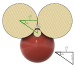
\includegraphics[width=8cm]{media/ang.png}
\end{center}

El ángulo $\alpha$ es determinante para el cálculo de la razón de radio, así:

$$\tan \left(\alpha\right) = \frac{\text{CO}}{\text{CA}} = \frac{1/2}{\sqrt{2}/2} = \frac{1}{\sqrt{2}}, \qquad \qquad \boxed{\alpha = \arctan\left( \frac{1}{\sqrt{2}} \right) = 35.26 \degree}$$

La razón de radios puede ser obtenida de la relación siguiente:

$$\cos \left(\alpha\right) = \frac{\text{CA}}{\text{H}} = \frac{r_-}{r_- + r_+}$$

$$r_+ \cos \left(\alpha\right) + r_- \cos \left(\alpha\right) = r_-$$

$$r_+ \cos \left(\alpha\right) = r_- \left(1 - \cos \left(\alpha\right)\right)$$

$$\frac{r_+}{r_-} = \frac{1 - \cos \left(\alpha\right)}{\cos \left(\alpha\right)}$$

$$\boxed{\frac{r_+}{r_-} \approx 0.225}$$